\documentclass[12pt]{article}

\usepackage[total={6.5in,8.75in}, top=2.4cm, left=2.4cm]{geometry}
\usepackage{lineno}
\usepackage{amsmath}
%\usepackage{amssymb}    % used for symbols in figure legends
\usepackage{graphicx}
\usepackage[round,colon,authoryear]{natbib}

\usepackage{bm}
\usepackage{float}
\usepackage{amsmath}
\usepackage{amsfonts}
\usepackage{hyperref}
\usepackage{verbatim}
\usepackage{soul}
\usepackage{color}
\usepackage{setspace}

\bibliographystyle{ecology} % kluwer, plos-natbib, pnas-natbib


\title{Ecological Distance in Spatial Capture-Recapture Models: Supplemental 
files}

\author{
{\bf J. Andrew Royle}\\
USGS Patuxent Wildlife Research Center, Laurel MD \\ \\
{\bf Richard B. Chandler} \\
USGS Patuxent Wildlife Research Center, Laurel MD\\ \\
{\bf Kimberly D. Gazenski} \\
USGS Patuxent Wildlife Research Center, Laurel MD\\ \\
{\bf Tabitha A. Graves} \\
Northern Arizona University, Flagstaff AZ \\ \\
}



\begin{document}

\maketitle

\date

\newpage

\linenumbers


\begin{spacing}{1.2}



\section*{Appendix 1: {\bf R} code for computing least-cost path
  distance and likelihood analysis of the SCR model}


As an example of the cost-weighted distance calculation consider the
following landscape comprised of 16 pixels with unit spacing
identified as follows, along with the pixel-specific cost:
\begin{center}
\begin{verbatim}
  pixel ID                 Cost
  1  5  9  13          100   1   1  1
  2  6 10  14          100 100   1  1
  3  7 11  15          100 100 100  1
  4  8 12  16          100 100   1  1
\end{verbatim}
\end{center}
Then we assigned low cost of 1 to ``good habitat'' pixels (or pixels
we think of as ``highly connected'' by virtue of being in good
habitat) and, conversely, we assign high cost (100) to ``bad
habitat''. So the shortest cost-weighted distance between pixels 5 and
9 in this example is just 1 unit, the shortest cost-distance between
pixels 5 and 10 is $\sqrt{2}(1+1)/2 = 1.414214$ units, the shortest
distance between pixels 4 and 8 is 100 units, while the shortest
cost-distance between 4 and 12 is 150.5. A tough one is: what is the
shortest distance between 7 and 16? An individual at pixel 7 can move
diagonal and pay $sqrt(2)*(100+1)/2 + 1 =72.41778$.  This simple cost
raster is shown in Fig. \ref{ecoldist.fig.raster}.

The {\bf R} commands to create a raster containing the pixel-specific
costs are given as follows for a simple $4\times 4$ raster containing
values either $z=1$ (good habitat) or $z=100$ (bad habitat):
\begin{verbatim}
r<-raster(nrows=4,ncols=4)
projection(r)<- "+proj=utm +zone=12 +datum=WGS84"
extent(r)<-c(.5,4.5,.5,4.5)
costs1<- c(100,100,100,100,1,100,100,100,1,1,100,1,1,1,1,1)
values(r)<-matrix(costs1,4,4,byrow=FALSE)
\end{verbatim}


\begin{figure}
\begin{center}
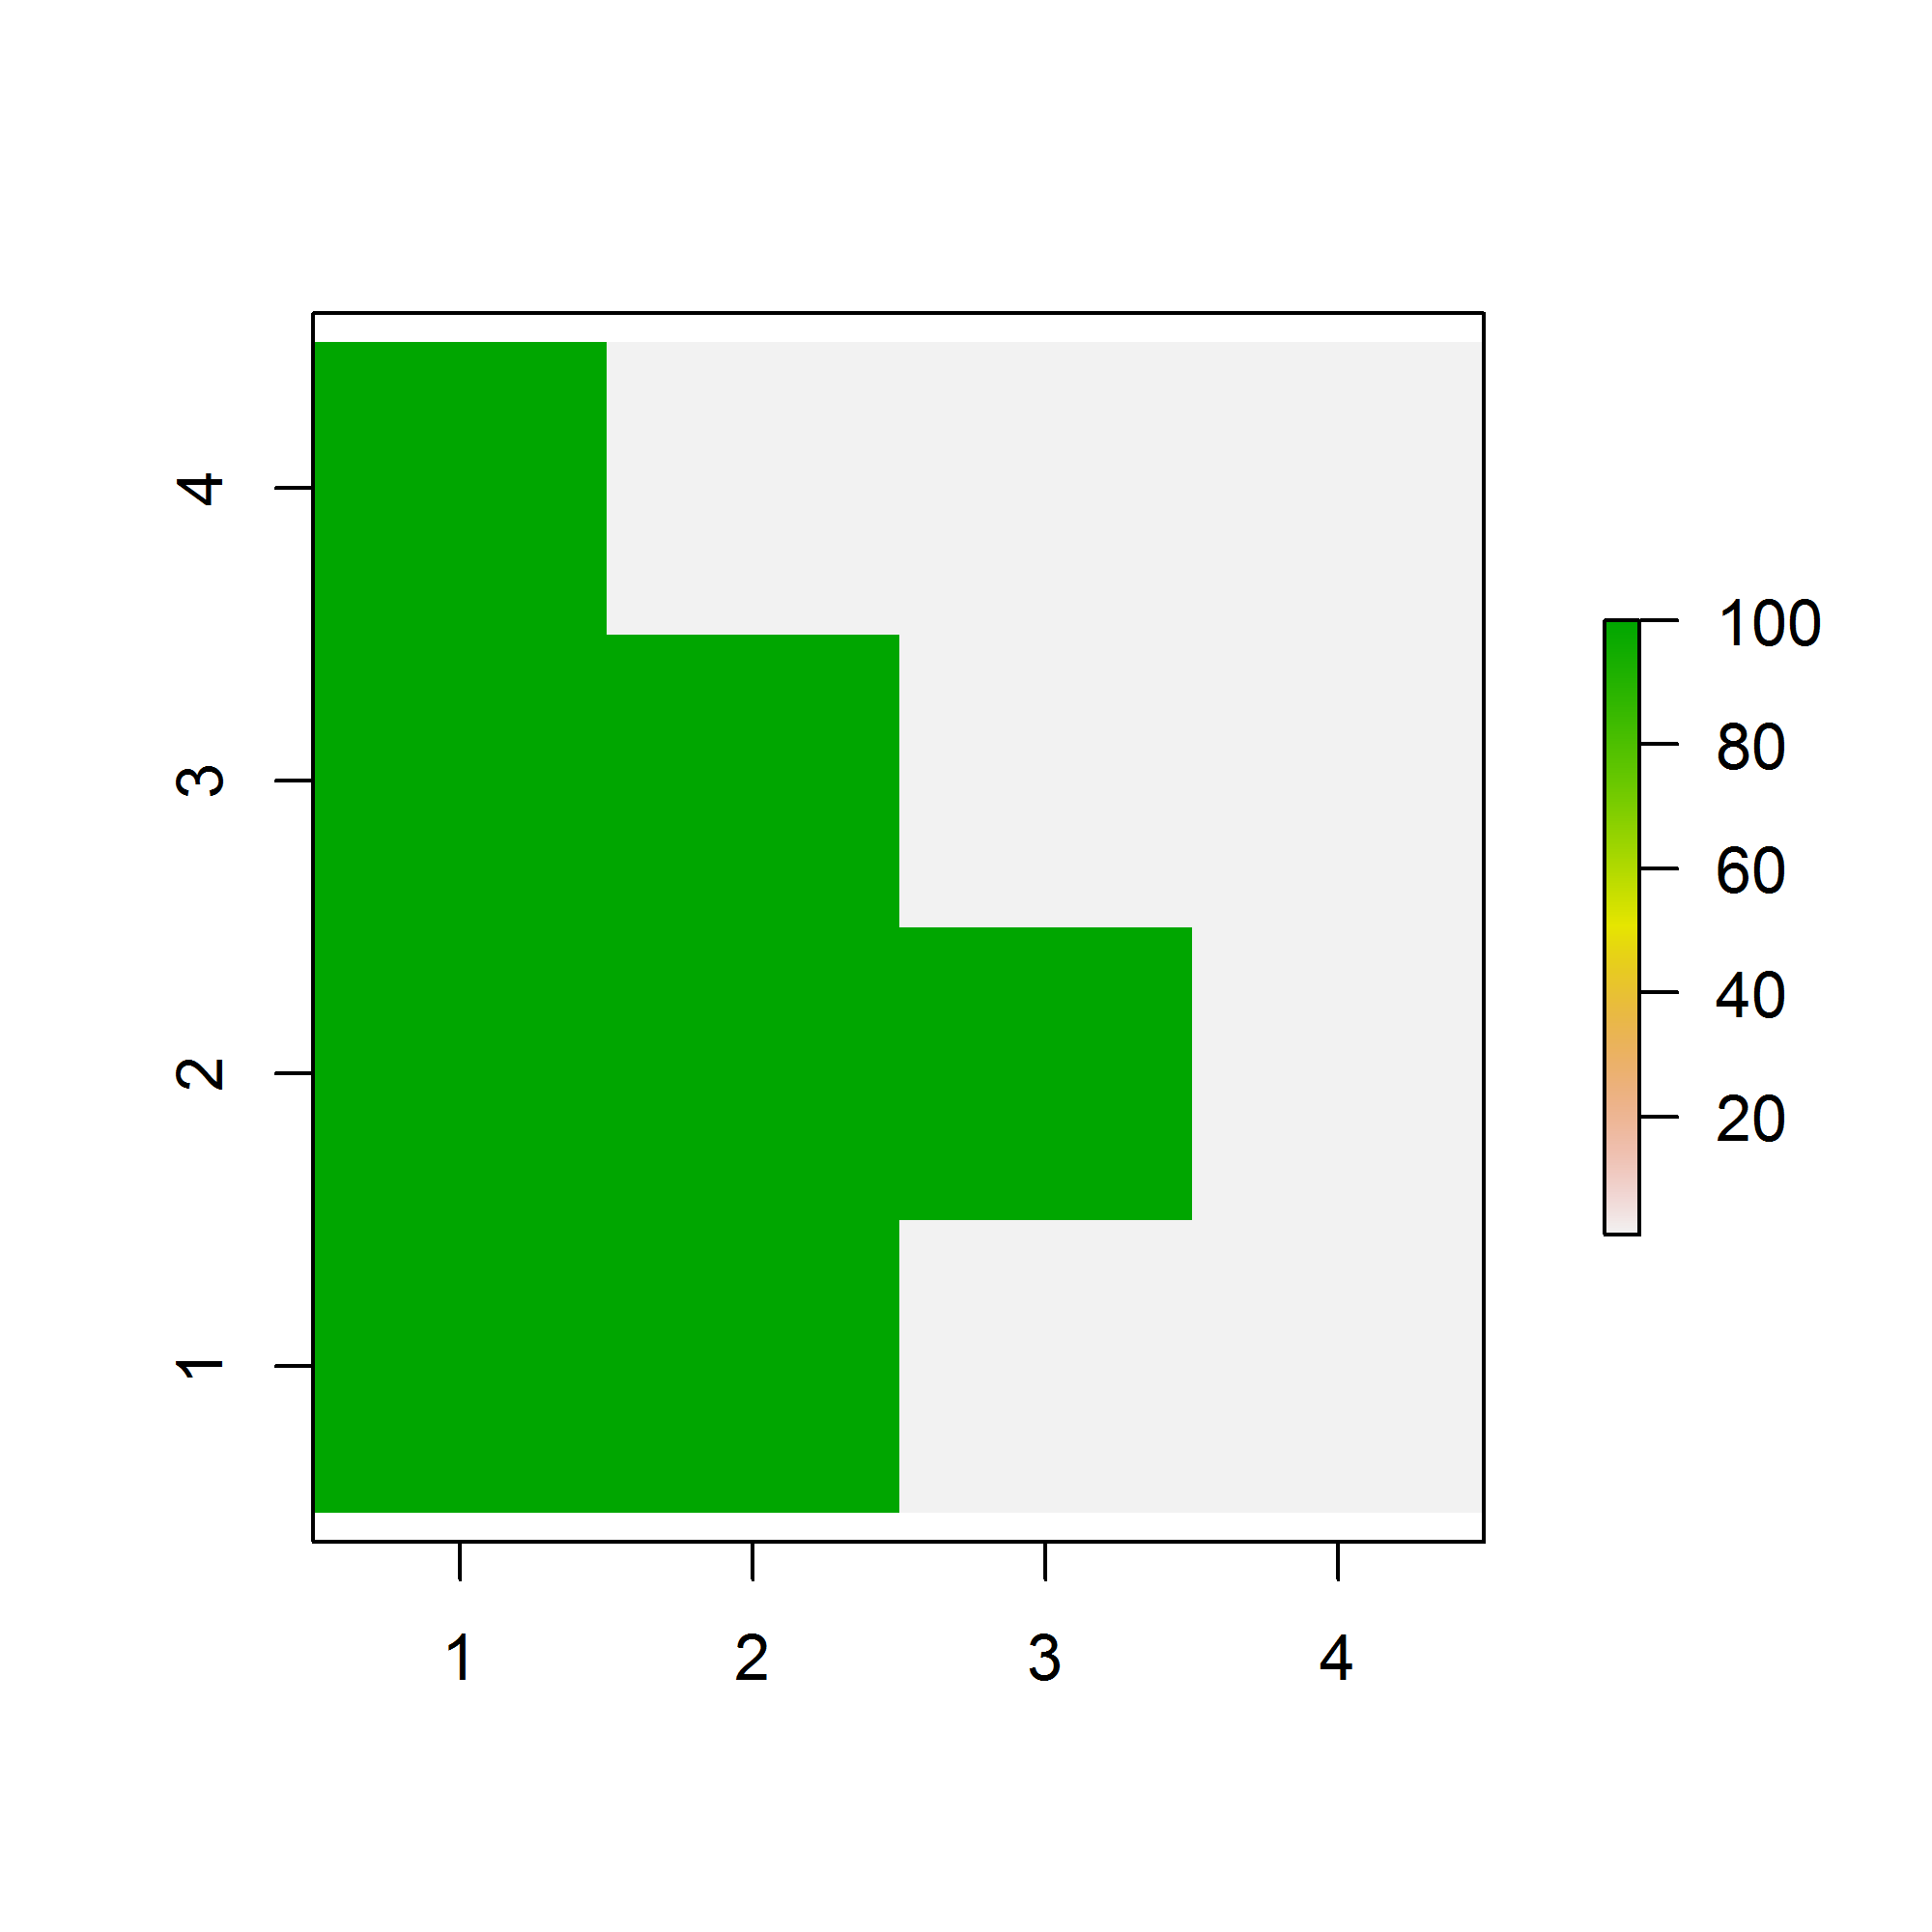
\includegraphics[height=3.25in,width=3.25in]{figs/raster_2values}
\end{center}
\caption{A $4 \times 4$ raster with cost = 1 (white) or 100 (shaded) to represent ease of movement across a pixel.}
\label{ecoldist.fig.raster}
\end{figure}


\begin{comment}
Now we can look at the result and see if it makes sense to us. Here we
print the first 4 columns of this distance matrix and illustration a
couple of examples of calculating the minimum cost-weighted distance
between points:
\begin{verbatim}
> outD[1:5,1:5]
         1         2        3        4         5
1   0.0000 100.00000 200.0000 205.2426  50.50000
2 100.0000   0.00000 100.0000 200.0000  71.41778
3 200.0000 100.00000   0.0000 100.0000 171.41778
4 205.2426 200.00000 100.0000   0.0000 154.74264
5  50.5000  71.41778 171.4178 154.7426   0.00000
\end{verbatim}
\end{comment}

Once the cost raster is created, the
least-cost path distances are computed with just a couple {\bf R}
commands, and those can be inserted directly into the likelihood
construction for an ordinary spatial capture-recapture model (Appendix
1). The {\bf R} package \mbox{\tt gdistance} uses the implementation
of Dijkstra's algorithm \citep{dijkstra:1959} found in the \mbox{\tt
  igraph} package \citep{csardi:2010}.  Using \mbox{\tt gdistance},
we define the incremental cost of moving from one pixel
to another as the distance-weighted {\it average} of the 2 pixel
costs.

To compute the least-cost path, or the minimimum cost-weighted
distances between every pixel and every other pixel, we make use of 
the helper functions \mbox{\tt transition}, which
calculates the cost of moving between neighboring pixels, and
\mbox{\tt geoCorrection} which modifies the costs of moving diagonally
by the additional distance, produce output which feeds into the
function \mbox{\tt costDistance} to compute the pair-wise distance
matrix. For that, we define the center points of each raster.  The
commands altogether are as follows:
\begin{comment}
# The transition function specifies that we'd like to use the mean of
# 2 neighboring pixels as the weight and then takes the inverse to convert
# the costs into conductances, which algorithms within gdistance and
# igraph require. We use the argument directions= 8 to specify that
# all 8 touching pixels are neighbors.)
\end{comment}
\begin{verbatim}
values(r)<-matrix(costs1,20,20,byrow=FALSE)
tr1<-transition(r,transitionFunction=function(x) 1/mean(x),directions=8)
tr1CorrC<-geoCorrection(tr1,type="c",multpl=FALSE,scl=FALSE)
pts<-cbind( sort(rep(1:4,4)),rep(4:1,4))
costs1<-costDistance(tr1CorrC,pts)
outD<-as.matrix(costs1)
\end{verbatim}


\section*{Appendix 2: Details for computing the marginal likelihood
  and obtaining the MLEs}


The key operation for computing the likelihood is solving the
2-dimensional integration problem to remove ${\bf s}$. There are some
general purpose {\bf R} packages that implement a number of
multi-dimensional integration routines including 
%\mbox{\tt adapt} \citep{genz_etal:2007} and  %% Not on CRAN anymore
\mbox{\tt R2Cuba} \citep{hahn_etal:2011}.
We won't rely on these extraneous {\bf R} packages but instead will
use perhaps less efficient methods in which we replace the integral
with a summation over an equal area mesh of points on the state-space
${\cal S}$ and explicitly evaluate the integrand at each point. We
invoke the rectangular rule for integration here in which the
integrand is evaluated on a regular grid of points of equal area and
then averaged.  Let $u=1,2,\ldots,nG$ index a grid of $nG$ points,
${\bf s}_{u}$, where the area of grid cell $u$ is constant.  In this
case, the integrand, i.e., the marginal pmf of ${\bf y}_{i}$, is
approximated by

\begin{equation}
         [{\bf y}_{i}|\alpha] = \frac{1}{nG} \sum_{u=1}^{nG}  [ {\bf
            y}_{i} |{\bf s}_u, \alpha]
\label{mle.eq.intlik}
\end{equation}

To deal with the fact that $N$ is unknown, there are two key issues
that need to be addressed.  First is that we don't observe the
``all-zero'' encounter histories (i.e., $y_{ij} = 0$ for all $j$)
corresponding to uncaptured individuals, so we have to make sure we
compute the probability for that all zero encounter history which we
do operationally by tacking a row of zeros onto the encounter history
matrix. We include the number of such all-zero encounter histories as
an unknown parameter of the model, which we label $n_{0}$.  In
addition, we have to be sure to include a combinatorial term to
account for the fact that of the $n$ observed individuals there are
${N \choose n}$ ways to realize a sample of size $n$. The
combinatorial term involves the unknown $n_{0}$ and thus it must be
included in the likelihood.

To compute the integral requires that the bounds of integration are
specified, which is equivalent to prescribing the state-space of the
underlying point process, i.e., ${\cal S}$. Given ${\cal S}$, density
is
computed as $D({\cal S}) = N/||{\cal S}||$. In our simulation study
below we report $N$ as the two are equivalent summaries of the data
set once the state-space is fixed.

We wrote an {\bf R} function to evaluate the likelihood which we optimize
using the {\bf R} function \mbox{\tt nlm}.
The {\bf R} code is given as a script in the Appendix where we also
provide functions for simulating data and carrying-out a simulation study.



\section*{Appendix 3: {\bf R} code for obtaining MLEs and the
  simulation study}

{\small
\begin{verbatim}
### Source all of the utility functions at the end of this script before
### running any of the code. 
###
###

### We require 3 R libraries
library("shapefiles")
library("gdistance")
library("raster")

###
### following block of code creates a "patchy" looking covariate to use
### in our cost function. It uses a standard method for generating a correlated
### multivariate normal vector of length, in this case, 400 (one value for each
### pixel). One can use any correlation function here but we chose a standard
### exponential model with range parameter 0.5
###png("raster_krige.png",width=5,height=5, units="in", res=400)
par(mfrow=c(1,1))
set.seed(12)
r<-raster(nrows=20,ncols=20)
projection(r)<- "+proj=utm +zone=12 +datum=WGS84"
extent(r)<-c(.5,4.5,.5,4.5)
delta<- (4.5-.5)/20
gx<- seq(.5 + delta/2, 4.5-delta/2,,20)
gy<- rev(gx)
gx<-sort(rep(gx,20))
gy<-rep(gy,20)
grid<-cbind(gx,gy)
Dmat<-as.matrix(dist(grid))
V<-exp(-Dmat/.5)
z<-t(chol(V))%*%rnorm(400)
z<- (z-mean(z))/sqrt(var(as.vector(z)))
#values(r)<-rot(rot(rot(matrix(z,20,20,byrow=TRUE))))
#values(r)<-(matrix(z,20,20,byrow=FALSE))
values(r)<-matrix(z,20,20,byrow=FALSE)
spatial.plot(grid,z)
par(mfrow=c(2,1))
plot(r)
####dev.off()
covariate.patchy<- z*sqrt(1.68) + .168   #approx. same scale as systematic covariate below
values(r)<-matrix(covariate.patchy,20,20,byrow=FALSE)
covariate.patchy<- r
class(covariate.patchy)

##
## build systematic covariate
## defined here as a trend from NW to SE
##
cost<-matrix(NA,nrow=20,ncol=20)
cost<-row(cost)+col(cost)
covariate.trend<- (cost-20)/10
values(r)<-matrix(covariate.trend,20,20,byrow=FALSE)
covariate.trend<-r
class(covariate.trend)


###
### generate Pr(encounter) for all pixels, for hypothetical traps in every other pixel
###  
### sigma = a bivariate normal home range parameter -- use different values to
### see how this looks
### alpha0 = intercept of detection prob. model
### alpha1 = coefficient on "distance" -- derived from "sigma"
### alpha2 = coefficient on covariate used in cost function
###
alpha2<- 1
alpha0<- -2   
sigma<-.25
alpha1<- 1/(2*sigma*sigma)
gx<- seq(.5 + delta/2, 4.5-delta/2,,20)
gy<- rev(gx)
gx<-sort(rep(gx,20))
gy<-rep(gy,20)
grid2<-cbind(gx,gy)
D<-e2dist(grid,grid2)
## Here is the stationary and isotropic detection model:
probcap<-plogis(alpha0)*exp(-alpha1*D*D)
## spatial.plot is a utility function (end of this script)
spatial.plot(grid2,probcap[1,])

###
### Set one of the cost functions -- either covariate.trend or covariate.patchy
###
cost<- exp(alpha2*covariate.patchy)
values(r)<-values(cost) ###matrix(cost,20,20,byrow=FALSE)
tr1<-transition(r,transitionFunction=function(x) 1/mean(x),directions=8)
tr1CorrC<-geoCorrection(tr1,type="c",multpl=FALSE,scl=FALSE)
costs1<-costDistance(tr1CorrC,grid,grid2)
outD<-as.matrix(costs1)
probcap<-plogis(alpha0)*exp(-alpha1*outD*outD)

###
### The following block of code will plot the "space usage" by 6 individuals with
### activity centers selected arbitrarily. You can plot this for any hypothetical
### individual if you wish
###png("home_ranges.png",width=5,height=8, units="in", res=400)
par(mfrow=c(3,2),mar=c(2,2,2,2))
#spatial.plot(grid2,probcap[63,])
#spatial.plot(grid2,probcap[76,])
values(r)<-matrix(probcap[63,],20,20,byrow=FALSE)
image(r,col=terrain.colors(10),axes=FALSE)
points(matrix(grid[63,],nrow=1),pch=20,cex=2)
values(r)<-matrix(probcap[76,],20,20,byrow=FALSE)
#plot(r,axes=FALSE)
image(r,col=terrain.colors(10),axes=FALSE)
points(matrix(grid[76,],nrow=1),pch=20,cex=2)


#spatial.plot(grid2,probcap[183,])
#spatial.plot(grid2,probcap[196,])
#spatial.plot(grid2,probcap[363,])
#spatial.plot(grid2,probcap[376,])
values(r)<-matrix(probcap[183,],20,20,byrow=FALSE)
image(r,col=terrain.colors(10),axes=FALSE)
points(matrix(grid[183,],nrow=1),pch=20,cex=2)

values(r)<-matrix(probcap[196,],20,20,byrow=FALSE)
image(r,col=terrain.colors(10),axes=FALSE)
points(matrix(grid[196,],nrow=1),pch=20,cex=2)

values(r)<-matrix(probcap[363,],20,20,byrow=FALSE)
image(r,col=terrain.colors(10),axes=FALSE)
points(matrix(grid[363,],nrow=1),pch=20,cex=2)

values(r)<-matrix(probcap[376,],20,20,byrow=FALSE)
image(r,col=terrain.colors(10),axes=FALSE)
points(matrix(grid[376,],nrow=1),pch=20,cex=2)

#####dev.off()




###
### R commands to carry-out the simulations. MUST SOURCE likelihood function first -- SEE BELOW
### This takes 1-2 days to run for nsims=100
###
###

nsims<-50

simout.low.N100<-sim.fn(N=100,nsim=nsims,alpha0=-2,sigma=.5,K=5,covariate=covariate.trend)
simout.low.N200<-sim.fn(N=200,nsim=nsims,alpha0= -2, sigma=.5,K=5,covariate=covariate.trend)
simout.reallylow.N100<-sim.fn(N=100,nsim=nsims,alpha0=-2,sigma=.5,K=3,covariate=covariate.trend)
simout.reallylow.N200<-sim.fn(N=200,nsim=nsims,alpha0= -2, sigma=.5,K=3,covariate=covariate.trend)
simout.high.N100<-sim.fn(N=100,nsim=nsims,alpha0=-2,sigma=.5,K=10,covariate=covariate.trend)
simout.high.N200<-sim.fn(N=200,nsim=nsims,alpha0= -2, sigma=.5,K=10,covariate=covariate.trend)

###
### R commands to summarize the simulation output
###
mat<-matrix(NA,nrow=9,ncol=10)
for(i in 1:3){
mat[i,1:5]<- smy.fn(exp(simout.reallylow.N100[[i]][,3]) + simout.reallylow.N100[[i]][,5])
mat[i,6:10]<- smy.fn(exp(simout.reallylow.N200[[i]][,3]) + simout.reallylow.N200[[i]][,5])
mat[3+i,1:5]<- smy.fn(exp(simout.low.N100[[i]][,3]) + simout.low.N100[[i]][,5])
mat[3+i,6:10]<- smy.fn(exp(simout.low.N200[[i]][,3]) + simout.low.N200[[i]][,5])
mat[6+i,1:5]<- smy.fn(exp(simout.high.N100[[i]][,3]) + simout.high.N100[[i]][,5])
mat[6+i,6:10]<- smy.fn(exp(simout.high.N200[[i]][,3]) + simout.high.N200[[i]][,5])
}

###
### 
### Using the "patchy" cost function execute these commands
###
###

simout.low.N100.k<-sim.fn(N=100,nsim=nsims,alpha0=-2,sigma=.5,K=5,covariate=covariate.patchy)
simout.low.N200.k<-sim.fn(N=200,nsim=nsims,alpha0= -2, sigma=.5,K=5,covariate=covariate.patchy)
simout.reallylow.N100.k<-sim.fn(N=100,nsim=nsims,alpha0=-2,sigma=.5,K=3,covariate=covariate.patchy)
simout.reallylow.N200.k<-sim.fn(N=200,nsim=nsims,alpha0= -2, sigma=.5,K=3,covariate=covariate.patchy)
simout.high.N100.k<-sim.fn(N=100,nsim=nsims,alpha0=-2,sigma=.5,K=10,covariate=covariate.patchy)
simout.high.N200.k<-sim.fn(N=200,nsim=nsims,alpha0= -2, sigma=.5,K=10,covariate=covariate.patchy)

###
### R commands to summarize the simulation output
###
mat.k<-matrix(NA,nrow=9,ncol=10)
for(i in 1:3){
mat.k[i,1:5]<- smy.fn(exp(simout.reallylow.N100.k[[i]][,3]) + simout.reallylow.N100.k[[i]][,5])
mat.k[i,6:10]<- smy.fn(exp(simout.reallylow.N200.k[[i]][,3]) + simout.reallylow.N200.k[[i]][,5])
mat.k[3+i,1:5]<- smy.fn(exp(simout.low.N100.k[[i]][,3]) + simout.low.N100.k[[i]][,5])
mat.k[3+i,6:10]<- smy.fn(exp(simout.low.N200.k[[i]][,3]) + simout.low.N200.k[[i]][,5])
mat.k[6+i,1:5]<- smy.fn(exp(simout.high.N100.k[[i]][,3]) + simout.high.N100.k[[i]][,5])
mat.k[6+i,6:10]<- smy.fn(exp(simout.high.N200.k[[i]][,3]) + simout.high.N200.k[[i]][,5])
}


#
# to do a single run you have to define a few things and then execute the code within the "sim.fn" below
#
covariate<-covariate.patchy
N<-200
alpha0<- -2
sigma<- .5
K<- 5

sim.fn<-function(N=200,nsim=100,alpha0= -2, sigma=.5, K=5,covariate){
# input covariate as a RasterLayer
#
cl<-match.call()
set.seed(2013)
simout2<-simout1<-simout3<-matrix(NA,nrow=nsim,ncol=5)
alpha1<- 1/(2*sigma*sigma)

r<-raster(nrows=20,ncols=20)
projection(r)<- "+proj=utm +zone=12 +datum=WGS84"
extent(r)<-c(.5,4.5,.5,4.5)
alpha2<-1
cost<- exp(alpha2*covariate)
#values(r)<-matrix(cost,20,20,byrow=FALSE)
#par(mfrow=c(1,1))
#plot(r)
r<-cost    

## use max = doesn't count moving through boundary pixel
tr1<-transition(r,transitionFunction=function(x) 1/mean(x),directions=8)
tr1CorrC<-geoCorrection(tr1,type="c",multpl=FALSE,scl=FALSE)

xg<-seq(1,4,1)
yg<-4:1
pts<-cbind( sort(rep(xg,4)),rep(yg,4))
#costs1<-costDistance(tr1CorrC,pts)
#D<-as.matrix(costs1)

traplocs<-pts
points(traplocs,pch=20,col="red")
ntraps<-nrow(traplocs)


for(sim in 1:nsim){

S<-cbind(runif(N,.5,4.5),runif(N,.5,4.5))
D<-costDistance(tr1CorrC,S,traplocs)
probcap<-plogis(alpha0)*exp(-alpha1*D*D)
# now generate the encounters of every individual in every trap
Y<-matrix(NA,nrow=N,ncol=ntraps)
for(i in 1:nrow(Y)){
 Y[i,]<-rbinom(ntraps,K,probcap[i,])
}
Y<-Y[apply(Y,1,sum)>0,]

# raster has to be defined for state-space and ssbuffer = 0 only
n0<- N-nrow(Y)
frog<-nlm(intlik3ed,c(alpha0,alpha1,log(n0)),hessian=TRUE,y=Y,K=K,X=traplocs,
               distmet="euclid",covariate=covariate,alpha2=1)
simout1[sim,]<-c(frog$estimate,NA,nrow(Y))

frog<-nlm(intlik3ed,c(alpha0,alpha1,log(n0)),hessian=TRUE,y=Y,K=K,X=traplocs,
               distmet="ecol",covariate=covariate,alpha2=1)
simout2[sim,]<-c(frog$estimate,NA,nrow(Y))

frog<-nlm(intlik3ed,c(alpha0,alpha1,log(n0),-.3),hessian=TRUE,y=Y,K=K,X=traplocs,
               distmet="ecol",covariate=covariate,alpha2=NA)
simout3[sim,]<-c(frog$estimate,nrow(Y))
}
list(simout1=simout1,simout2=simout2,simout3=simout3,call=cl)

}

##
##
## UTILITY FUNCTIONS
## 
## PUT ALL OF THE OBJECTS BELOW INTO YOUR WORKSPACE
##
	
intlik3ed<-function(start=NULL,y=y,K=NULL,delta=.2,X=traplocs,
distmet="ecol",covariate,alpha2=NA){

if(is.null(K)) return("need sample size")
if(class(covariate)!="RasterLayer") {
 cat("make a raster out of this",fill=TRUE)
 return(NULL)

}
# do a check here that trap locations exist in same space as raster. 
# forthcoming

# build integration grid. This derives from the covariate raster
# i.e., potential values of s are the mid-point of each raster pixel
nc<-covariate@ncols
nr<-covariate@nrows
Xl<-covariate@extent@xmin
Xu<-covariate@extent@xmax
Yl<-covariate@extent@ymin
Yu<-covariate@extent@ymax
SSarea<- (Xu-Xl)*(Yu-Yl)
### ASSUMES SQUARE RASTER -- NEED TO GENERALIZE THIS
delta<- (Xu-Xl)/nc
xg<-seq(Xl+delta/2,Xu-delta/2,delta) 
yg<-seq(Yl+delta/2,Yu-delta/2,delta) 
npix.x<-length(xg)
npix.y<-length(yg)
area<- (Xu-Xl)*(Yu-Yl)/((npix.x)*(npix.y))
G<-cbind(rep(xg,npix.y),sort(rep(yg,npix.x)))
nG<-nrow(G)

if(distmet=="euclid")
D<- e2dist(X,G)  

if(distmet=="ecol"){
if(is.na(alpha2))
alpha2<-exp(start[4])

cost<- exp(alpha2*covariate)
tr1<-transition(cost,transitionFunction=function(x) 1/mean(x),directions=8)
tr1CorrC<-geoCorrection(tr1,type="c",multpl=FALSE,scl=FALSE)
D<-costDistance(tr1CorrC,X,G)
}

if(is.null(start)) start<-c(0,0,0,0)
alpha0<-start[1]
alpha1<-start[2]
n0<-exp(start[3])


probcap<- (exp(alpha0)/(1+exp(alpha0)))*exp(-alpha1*D*D)
Pm<-matrix(NA,nrow=nrow(probcap),ncol=ncol(probcap))
ymat<-y
ymat<-rbind(y,rep(0,ncol(y)))
lik.marg<-rep(NA,nrow(ymat))
for(i in 1:nrow(ymat)){
Pm[1:length(Pm)]<- (dbinom(rep(ymat[i,],nG),rep(K,nG),probcap[1:length(Pm)],log=TRUE))
lik.cond<- exp(colSums(Pm))
lik.marg[i]<- sum( lik.cond*(1/nG) )  
}                                                 
nv<-c(rep(1,length(lik.marg)-1),n0)
part1<- lgamma(nrow(y)+n0+1) - lgamma(n0+1)
part2<- sum(nv*log(lik.marg))
out<-  -1*(part1+ part2)
attr(out,"SSarea")<- SSarea
out
}

image.scale <-
function (z, col, x, y = NULL, size = NULL, digits = 2, labels = c("breaks", 
    "ranges"))
{
    # sort out the location
    n <- length(col)
    usr <- par("usr")
    mx <- mean(usr[1:2]); my <- mean(usr[3:4])
    dx <- diff(usr[1:2]); dy <- diff(usr[3:4])
    if (missing(x))
        x <- mx + 1.05*dx/2	# default x to right of image
    else if (is.list(x)) {
        if (length(x$x) == 2) 
          size <- c(diff(x$x), -diff(x$y)/n)
        y <- x$y[1]
        x <- x$x[1]
    } else x <- x[1]
    if (is.null(size))
        if (is.null(y)) {
          size <- 0.618*dy/n	# default size, golden ratio
          y <- my + 0.618*dy/2	# default y to give centred scale
        } else size <- (y-my)*2/n
    if (length(size)==1)
        size <- rep(size, 2)	# default square boxes
    if (is.null(y))
        y <- my + n*size[2]/2
    # draw the image scale
    i <- seq(along = col)
    rect(x, y - i * size[2], x + size[1], y - (i - 1) * size[2], 
        col = rev(col), xpd = TRUE)
    # sort out the labels
    rng <- range(z, na.rm = TRUE)
    bks <- seq(from = rng[2], to = rng[1], length = n + 1)
    bks <- formatC(bks, format="f", digits=digits)
    labels <- match.arg(labels)
    if (labels == "breaks")
        ypts <- y - c(0, i) * size[2]
    else {
        bks <- paste(bks[-1], bks[-(n+1)], sep = " - ")
        ypts <- y - (i - 0.5) * size[2]
    }
    text(x = x + 1.2 * size[1], y = ypts, labels = bks, adj =
        ifelse(size[1]>0, 0, 1), xpd = TRUE) 
}

spatial.plot <-
function(x,y,add=TRUE,cx=1){
 nc<-as.numeric(cut(y,20))
if(!add) plot(x,pch=" ")
 points(x,pch=20,col=terrain.colors(20)[nc],cex=cx)
image.scale(y,col=terrain.colors(20))

}
e2dist <- function (x, y)
{
    i <- sort(rep(1:nrow(y), nrow(x)))
    dvec <- sqrt((x[, 1] - y[i, 1])^2 + (x[, 2] - y[i, 2])^2)
    matrix(dvec, nrow = nrow(x), ncol = nrow(y), byrow = F)
}
smy.fn <-
function(x){
c(mean(x),sqrt(var(x)),quantile(x,c(0.025,0.50,0.975)))
}
\end{verbatim}
}

\newpage


\section*{Appendix 4:  MLE summary statistics for reanalysis of the
  systematic landscape}


For both landscapes and all simulation conditions (levels of $K$ and
$N$) the average sample sizes of individuals captured are given in
Table~\ref{tab.samplesize}.  


\begin{table}[ht]
\centering
\caption{
Expected sample sizes of captured individuals under each configuration of
$N$ (population size for the prescribed state-space) and $K$ (number of replicate samples).
}
\begin{tabular}{l|rrrr}
 & \multicolumn{2}{c}{Systematic} & \multicolumn{2}{c}{Patchy}  \\
    & N=100 &  N=200  &   N=100 &  N=200  \\ \hline
K=3 &  38.69 &   78.17  &   37.30 &   74.93  \\
K=5 &  51.10 &  103.18  &   51.89 &  103.71 \\
K=10&  65.81 &  132.39  &   69.44 &  138.76 \\
\end{tabular}
\label{tab.samplesize}
\end{table}



\begin{table}[ht]
{\small
\caption{Simulation results for estimating population size $N$ for a prescribed state-space with
$N=100$ or $N=200$ and various levels of replication ($K$) chosen to affect the observed sample
size of individuals. These results correspond to those of the
systematic landscape in Table 2 except with the traps
moved 0.5 units in from the boundary of the raster.
Each grouping of 3 rows (for a given value of $K$) summarizes the
performance of $\hat{N}$ under 3 distance models: (1) A model in which
Euclidean distance was used (``euclid''); (2) A model in which the
least-cost path distance was used, with the coefficient of the cost
function fixed (``lcp/known''); and (3) A model in which the
coefficient was estimated (``lcp/est''). The summary statistics of the
sampling distribution reported are the mean, standard deviation
(``SD'') and quantiles (0.025, 0.50, 0.975).
}
{\bf Systematic trend raster:} \\
\begin{tabular}{l|rrrrr|rrrrr}
         & \multicolumn{5}{c}{N=100   } & \multicolumn{5}{c}{N=200  }  \\
         &   mean &  SD  & 0.025 & 0.50 & 0.975  & mean  & SD   & 0.025 & 0.50  & 0.975 \\ \hline
K=3      &        &      &       &      &        &       &      &       &       &       \\
euclid   &   84.48& 20.42& 51.16 & 81.51& 140.62 &163.70 &24.55 &126.64 &157.67 &223.63 \\
lcp/known&  104.14& 25.49& 65.67 &101.50& 173.19 &200.16 &29.27 &158.65 &191.04 &268.78\\
lcp/est  &  105.90& 26.19& 65.95 &103.40& 182.30 &201.34 &29.54 &161.88 &192.36 &268.98\\
K=5      &        &      &       &      &        &       &      &       &       &       \\
euclid   & 81.21  &11.33 &61.35  &79.20 & 98.86  &163.27 &13.06 &140.21 &162.97 &185.94\\
lcp/known& 99.93  &12.86 &76.97  &99.75 &117.76  &199.80 &16.60 &170.25 &198.23 &227.66\\
lcp/est  & 100.84 &13.15 &79.96  &99.51 &119.08  &200.25 &16.53 &168.88 &199.29 &227.39\\
K=10     &        &      &       &      &        &       &      &       &       &       \\
euclid   &  80.10 & 7.81 &66.45  &79.14 &93.33   &158.40 & 9.25 &142.74 &157.86 &173.18\\
lcp/known& 100.07 & 9.50 &82.99  &100.33&114.81  &197.62 &12.58 &171.95 &199.21 &217.19\\
lcp/est  & 100.10 & 9.88 &82.31  &100.91&116.27  &197.52 &13.03 &169.49 &200.68 &217.82\\ \hline
\end{tabular}
}
\label{tab.results3}
\end{table}






\begin{table}[ht]
\centering
\caption{
Mean of sampling distribution of the cost function parameter
$\alpha_{2}$ for the different simulation
conditions.  The simulation for the systematic landscape was repeated
with sample locations concentrated away from the boundary of the
landscape to avoid truncation bias in computing the integrated
likelihood. Results for that case are shown in rows 4-6.
}
\begin{tabular}{l|rrrr}
 & \multicolumn{2}{c}{Patchy} & \multicolumn{2}{c}{Systematic} \\
    & N=100 &  N=200  &   N=100 &  N=200  \\ \hline
K=3 &   1.05&    1.03 &     1.17 & 1.14 \\
K=5 &   1.02&    1.01 &     1.12 &1.12 \\
K=10&   1.01&    1.00 &     1.10 &1.08 \\ \hline
K=3    &       &         &     1.08 & 1.04 \\
K=5    &       &         &     1.02 & 1.02 \\
K=10    &       &         &     1.01 & 1.01 \\
\end{tabular}
\label{tab.results2}
\end{table}







\bibliography{../AndyRefs_alphabetized}


\end{spacing}

\end{document}






